%-----------------------------------------------
% Dateiname: Colophon.tex
% Autor    : Stefano Kowalke <blueduck@gmx.net>
% Lizenz   : BSD
%-----------------------------------------------
\thispagestyle{empty}
\vspace*{\fill}
\begin{flushleft}
    \sffamily
    \footnotesize
    \noindent
Dieses Dokument wurde am \today\ mit \InfoLaTeX\ gesetzt.
    \par\bigskip\noindent
    \begin{tabular}{ll}
Schrift: & {Palatino 10pt}\\
Typographie: & \KOMAScriptVersion\\
System: & \InfoTeX\ auf OSX 10.8\\
Editor: & Mou 0.8.5 beta und VIM 7.4 \\
    \end{tabular}
    \par\bigskip\noindent
    {Es steht unter der \textbf{Creative Commons Namensnennung – Weitergabe unter gleichen Bedingungen 4.0 International Lizenz}} und kann unter \url{https://github.com/Konafets/thesis} heruntergeladen werden.
    \begin{figure}[h!]
        \centering
        \includegraphics[scale=0.75]{by-sa.eps}
     \end{figure}\\
     Der für diese Thesis entstandene Prototyp steht unter der \textbf{GNU General Public License version 2 oder neuer} \url{http://www.gnu.org/licenses/gpl-2.0.html} und ist unter \url{https://github.com/Konafets/ext-doctrine_dbal} zu finden.

     TYPO3 CMS steht unter der \textbf{GNU General Public License version 2 oder neuer} \url{http://www.gnu.org/licenses/gpl-2.0.html}. Die modifizierte Version ist unter \url{https://github.com/Konafets/TYPO3CMSDoctrineDBAL} zu finden.
     \\[1\baselineskip]

	 Das Latex-Template basiert auf der ClassicThesis von André Miede zu finden unter \url{http://www.miede.de/index.php?page=classicthesis}. Es steht unter der \textbf{GNU General Public License} \url{http://www.gnu.org/copyleft/gpl.html}.
     \\[1\baselineskip]

	 \textit{The Joy of Programming with Bob Ross} von Abstruse Goose zu finden unter \url{http://abstrusegoose.com/467} steht unter der Lizenz \textbf{Attribution-NonCommercial 3.0 United States (CC BY-NC 3.0 US)} \url{http://creativecommons.org/licenses/by-nc/3.0/us/}.
     \\[1\baselineskip]
	 \textit{Exploits of a mom} von xkcd zu finden unter \url{http://xkcd.com/327/} steht unter der Lizenz \textbf{Attribution-NonCommercial 2.5 Generic (CC BY-NC 2.5)} \url{http://creativecommons.org/licenses/by-nc/2.5/}.
\end{flushleft}
\normalsize
